% Fig. 1 (Applied Energy) -- reference heat-rejection system and supplemental cooling options.
% Final width 190 mm, fonts 9/8/7.5 pt, relative positioning only,
% 3 hues + grey, line style carries the meaning in black and white.
\documentclass[border=1mm]{standalone}
\usepackage[T1]{fontenc}
\usepackage{helvet}
\usepackage{textcomp}
\renewcommand{\familydefault}{\sfdefault}
\usepackage{tikz}
\usetikzlibrary{positioning,calc,arrows.meta,backgrounds,fit,shapes.geometric}
\definecolor{dryfill}{HTML}{EAF2F8}\definecolor{dryline}{HTML}{24557A}
\definecolor{wetfill}{HTML}{E5F3ED}\definecolor{wetline}{HTML}{176B50}
\definecolor{compfill}{HTML}{FFF1DD}\definecolor{compline}{HTML}{925400}
\definecolor{itfill}{HTML}{F3F4F5}\definecolor{itline}{HTML}{4B5055}
\definecolor{ink}{HTML}{222222}
\newcommand{\lone}{\fontsize{9}{10.6}\selectfont\bfseries}
\newcommand{\ltwo}{\fontsize{8}{9.5}\selectfont}
\newcommand{\lthree}{\fontsize{7.5}{9}\selectfont}
\newcommand{\dC}{\,\textdegree C}
\begin{document}
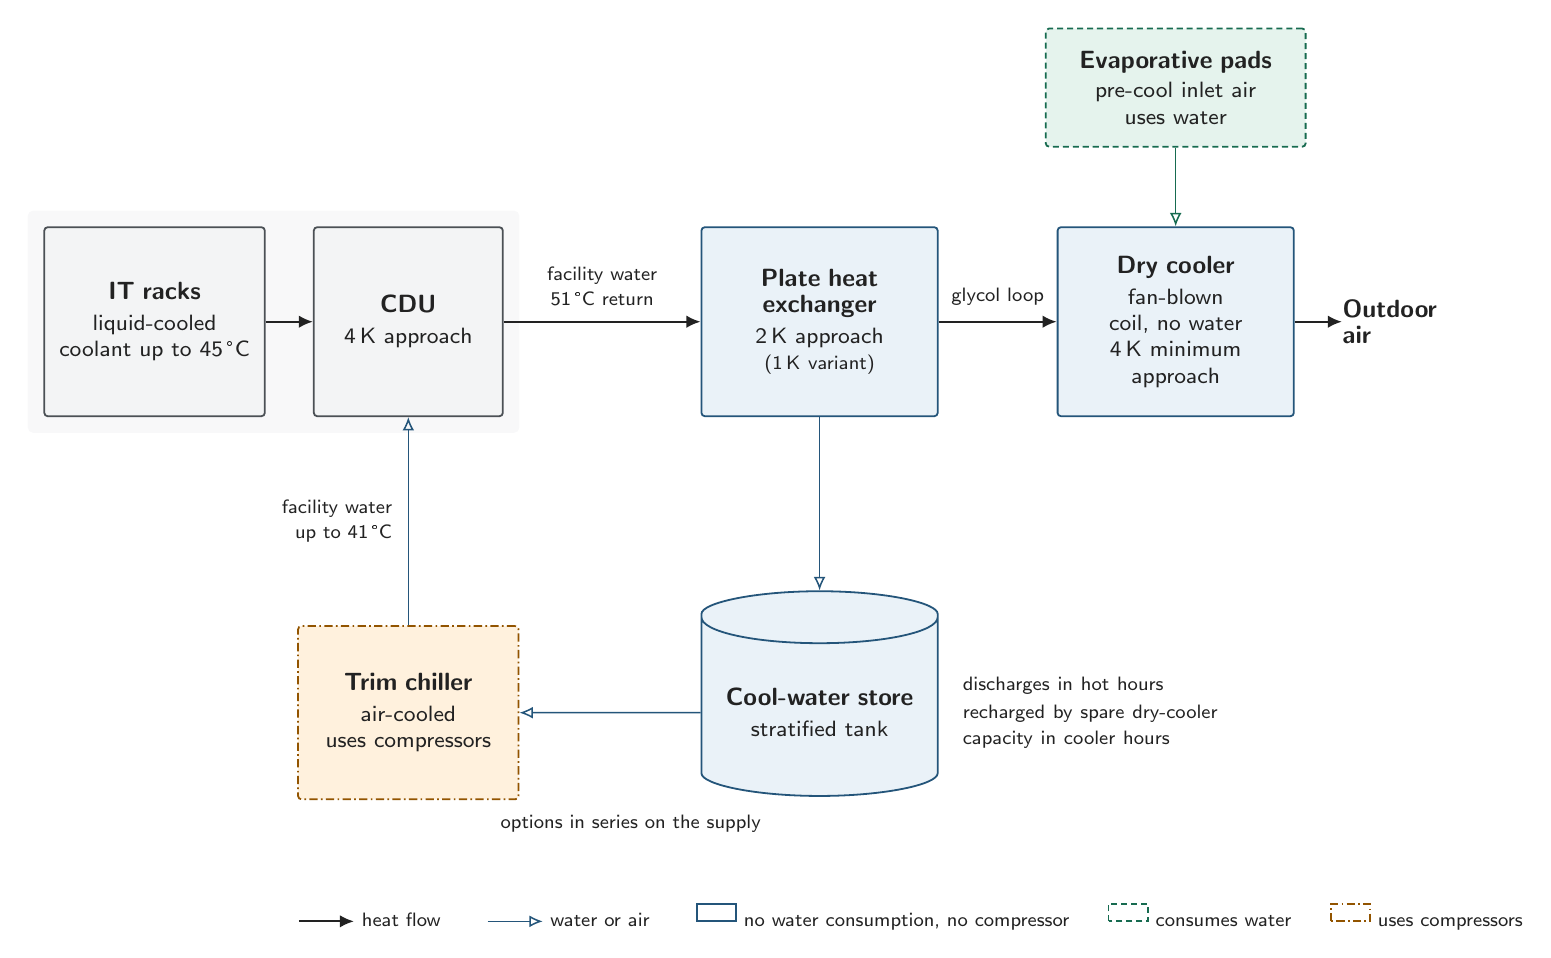
\begin{tikzpicture}[
  font=\ltwo, text=ink, execute at begin node={\hyphenpenalty=10000\exhyphenpenalty=10000},
  unit/.style={rounded corners=1.2pt, align=center, line width=0.65pt, minimum height=24mm, inner sep=1.5mm},
  itbox/.style={unit, draw=itline, fill=itfill},
  drybox/.style={unit, draw=dryline, fill=dryfill},
  wetbox/.style={unit, draw=wetline, fill=wetfill, dash pattern=on 2.2pt off 1.4pt},
  compbox/.style={unit, draw=compline, fill=compfill, dash pattern=on 3pt off 1.2pt on 0.6pt off 1.2pt},
  heat/.style={draw=ink, line width=0.8pt, -{Latex[length=1.8mm,width=1.6mm]}},
  supply/.style={draw=dryline, line width=0.55pt, -{Latex[open,length=1.7mm,width=1.5mm]}},
  inlet/.style={draw=wetline, line width=0.55pt, -{Latex[open,length=1.7mm,width=1.5mm]}},
]
% ---------------- row 2: heat path, left to right ----------------
\node[itbox, text width=25mm] (racks) {{\lone IT racks}\\[0.6mm]liquid-cooled\\coolant up to 45\dC};
\node[itbox, text width=21mm, right=6mm of racks] (cdu) {{\lone CDU}\\[0.6mm]4\,K approach};
\node[drybox, text width=27mm, right=25mm of cdu] (hx) {{\lone Plate heat\\exchanger}\\[0.6mm]2\,K approach\\{\lthree (1\,K variant)}};
\node[drybox, text width=27mm, right=15mm of hx] (dc) {{\lone Dry cooler}\\[0.6mm]fan-blown coil, no water\\4\,K minimum approach};
\node[right=6mm of dc, align=left, text width=15mm, inner sep=0pt] (air) {{\lone Outdoor\\air}};
% group IT racks + CDU
\begin{scope}[on background layer]
  \node[fit=(racks)(cdu), inner sep=2mm, fill=itfill!60, draw=none, rounded corners=2pt] {};
\end{scope}
% ---------------- row 1: evaporative pads above the dry cooler ----------------
\node[wetbox, text width=30mm, minimum height=15mm, above=10mm of dc] (pads) {{\lone Evaporative pads}\\[0.4mm]pre-cool inlet air\\uses water};
% ---------------- row 3: supply-water series segment ----------------
\node[drybox, cylinder, shape border rotate=90, aspect=0.22, text width=27mm, minimum height=26mm, below=22mm of hx] (store)
  {{\lone Cool-water store}\\[0.6mm]stratified tank};
\node[compbox, text width=25mm, minimum height=22mm] (chiller) at (cdu |- store) {{\lone Trim chiller}\\[0.6mm]air-cooled\\uses compressors};
\node[below=2.5mm of $(chiller.south east)!0.5!(store.south west)$, anchor=north, inner sep=0pt, align=center, font=\lthree] {options in series on the supply};
\node[right=3mm of store, align=left, text width=48mm, inner sep=0pt] (note) {\lthree discharges in hot hours\\[0.3mm]recharged by spare dry-cooler\\capacity in cooler hours};
% ---------------- edges ----------------
\draw[heat] (racks) -- (cdu);
\draw[heat] (cdu) -- node[above=0.8mm, align=center, font=\lthree] {facility water\\51\dC{} return} (hx);
\draw[heat] (hx) -- node[above=0.8mm, font=\lthree] {glycol loop} (dc);
\draw[heat] (dc) -- (air);
\draw[supply] (hx.south) -- (store.north);
\draw[supply] (store.west) -- (chiller.east);
\draw[supply] (chiller.north) -- node[left=0.8mm, align=right, font=\lthree] {facility water\\up to 41\dC} (cdu.south);
\draw[inlet] (pads.south) -- (dc.north);
% ---------------- legend ----------------
\node[below=13mm of chiller.south west, anchor=north west, inner sep=0pt, align=left, font=\lthree] (leg) {%
  \tikz[baseline=-0.6ex]\draw[heat] (0,0) -- (7mm,0); heat flow\hspace{5mm}
  \tikz[baseline=-0.6ex]\draw[supply] (0,0) -- (7mm,0); water or air\hspace{5mm}
  \tikz[baseline=-0.6ex]\draw[dryline, line width=0.65pt] (0,0) rectangle (5mm,2.2mm); no water consumption, no compressor\hspace{4mm}
  \tikz[baseline=-0.6ex]\draw[wetline, line width=0.65pt, dash pattern=on 2.2pt off 1.4pt] (0,0) rectangle (5mm,2.2mm); consumes water\hspace{4mm}
  \tikz[baseline=-0.6ex]\draw[compline, line width=0.65pt, dash pattern=on 3pt off 1.2pt on 0.6pt off 1.2pt] (0,0) rectangle (5mm,2.2mm); uses compressors};
\end{tikzpicture}
\end{document}
